% !TEX root = ../thesis.tex

\chapter{Analytická časť}\label{ch:current-state}

\section{Klasifikácia objektov}

Pod názvom klasifikácia objektov môžeme chápať úlohu, ktorá identifikuje a kategorizuje objekty v obrázku s vopred definovanými triedami.
Klasifikácia objektov je typicky vykonávaná technológiami strojového učenia, kde model je trenovaný na vybranej dátovej sade obrázkov a ich priradenie do označených tried.
Trenovací model môže byť použitý na klasifikovanie nových obrázkov priradením označenia triedy na základe ich naučených vlasností.
Použitie klasifikácie objektov je zahrnuté napr. pri rozpoznávaní dopravných značiek alebo identifikáciu rastliny na obrázku. \cite{kili}

\begin{figure}[H]
    \centering
    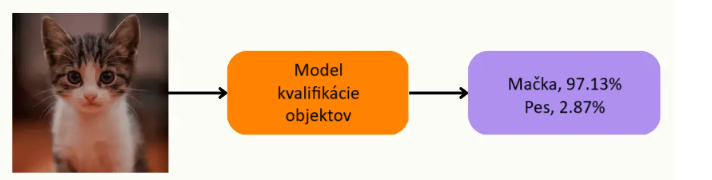
\includegraphics[width=1\linewidth]{figures/OCmodel.png}
    \caption{Zreťazenie klasifikácie objektov \label{OCmodel}}
    \label{fig:enter-label}
\end{figure}

\section{Detekcia objektov}

Detekcia objektov je z pohľadu počítača úloha, ktorá identifikuje a lokalizuje objekty na základe preddefinovaných triedach vo vstupných obrázkov.
S vývojom neurónových sietí, detekcia objektov dosiahla veľmi sľubné výsledky.
Existuje pár modelov a algoritmov ako sú R-CNN, Faster R-CNN, YOLO a SSD, ktoré boli vyvinuté na detekciu objektov.
Tieto algoritmy a modely sa používajp v rôznych aplikáciách, ako je samojazdiace autá, sledovacie systémy a sledovanie objektov.

\begin{figure}[H]
    \centering
    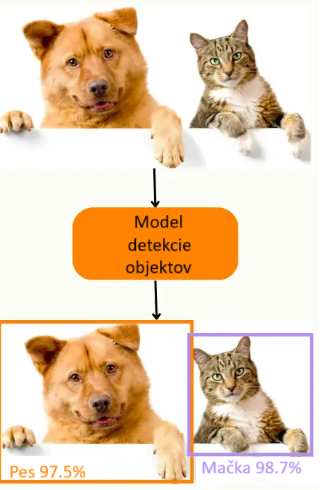
\includegraphics[width=0.45\linewidth]{figures/ODmodel.png}
    \caption{Zreťazenie detekcie objektov \label{ODmodel}}
    \label{fig:enter-label}
\end{figure}

\section{YOLO}

YOLO (You Only Look Once) je algoritmus detekcie objektov v reálnom čase, vyvinutý v roku 2015 dvojicou autorov Joseph Redmon a Ali Farhadi.
Ide o jednostupňový detektor objektov, ktorý využíva konvolučnú neurónovú sieť (CNN) na prepovedanie ohraničujúcich políčok a prevdepodobností tried objektov vo vstupných obrázkoch.

Algoritmus YOLO rozdeľuje vstupný obrázok na mriežku buniek a pre každú bunku predpovedá pravdepodobnosť prítomnosti objektu a súradnice ohraničujúceho rámčeka objektu a prepovedá tiež triedu objektu.
Na rozdiel od dvojstupňovových detektorov objektov, ako je R-CNN a jeho variantov, YOLO spracováva celý obraz v jednom priechode, vďaka čomu je rýchlejší a efektívnejší.

YOLO bolo vyvinuté v niekoľkých verziách od YOLOv1 až po najnovšie YOLOv12. Každá verzia bola postavená na predchádzajúcej verzii s vylepšenými funkciami, ako je vylepšená presnosť, rýchlejšie spracovanie a lepšia manipulácia s malými predmetmi.

YOLO je široko používaný v rôznych aplikáciach, ako sú samoriadiace autá a sledovacie systémy.
Je tiež široko používaný na úlohy detekcie objektov v reálnom čase, ako je analýza videa v reálnom čase a video dohľad v reálnom čase.

\subsubsection{Princíp YOLO algoritmu}



\subsubsection{Výhody YOLO algoritmu}



\subsubsection{Nevýhody YOLO algoritmu}


\begin{figure}[H]
    \centering
    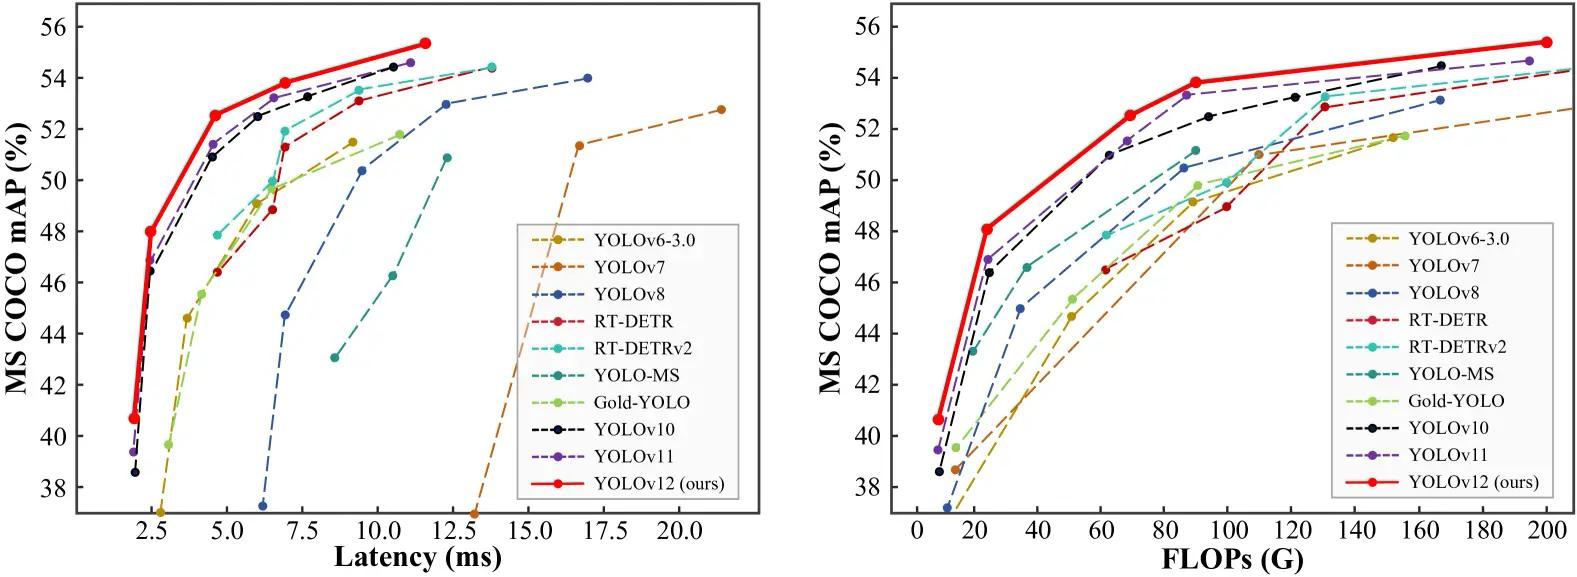
\includegraphics[width=1\linewidth]{figures/yolo.jpg}
    \caption{Porovnanie s ďalšimi známymi metódami pokiaľ ide o kompromisy latencie-presnosť (vľavo) a FLOP-presnosť (vpravo) \label{yolo}}
    \label{fig:enter-label}
\end{figure}

